% ARAGUAIA: A SAGA DE OSVALDÃO --------------------------------------------------------

\chapter{O JOGO -- ARAGUAIA: A SAGA DE OSVALDÃO}
\label{chap:araguaia-osvaldao}

Apresenta-se, neste capítulo, as etapas de desenvolvimento do jogo, norteadas pelo \textit{framework} desenvolvido pela equipe, apresentado na seção \ref{sec:desenvolvimento}. As seções abaixo apresentam cada etapa do modelo seguido, aplicadas ao jogo desenvolvido.

\section{Ambientação da Equipe}
\label{sec:ambientacao}

Nesta etapa, foram realizadas algumas reuniões e viagens para a capacitação da equipe de desenvolvimento do projeto, tanto em termos do assunto alvo -- Guerrilha do Araguaia, como das ferramentas para desenvolver o jogo (descritas na seção \ref{sec:ferramentas}). As viagens realizadas aos locais onde ocorreu a Guerrilha foram muito úteis para a coleta de dados a serem utilizados no jogo, principalmente imagens e vídeos, que revelaram características interessantes da fauna e flora da região. Após isso, fora definido o enredo do jogo, bem como o roteiro de algumas missões da primeira fase.

\addtocontents{toc}{\protect\setcounter{tocdepth}{1}}
\subsection{Início das Atividades}

As atividades iniciaram após a aprovação do programa de extensão ``Construção de Jogos Educativos e Implantação em Escolas Públicas da Cidade de Marabá", no Programa Institucional de Bolsas de Extensão (PIBEX) $2016$, que tem como um dos seus objetivos específicos ``Projetar e Implementar o jogo sobre a Guerrilha do Araguaia, tendo Osvaldão como personagem protagonista do enredo".

A equipe que projetou e implementou o jogo foi coordenada por um profissional da área de computação, com experiência em game \textit{design}, tendo já coordenado a construção de quatro jogos educativos que resultaram em publicações de artigos, dissertações de mestrado, TCCs e têm sido utilizados em escolas dos ensinos médio e fundamental. Um professor de história, estudioso da Guerrilha do Araguaia, e que também é escritor, tendo publicado um livro de contos, portanto ficção, livremente inspirado na memória social da Guerrilha (relatos de camponeses que conviveram com guerrilheiros e soldados do exército antes e durante o conflito armado). Três programadores, que trabalharam na implementação do jogo (game \textit{engine} e \textit{scripts}), e quatro artistas que trabalharam na elaboração e construção dos cenários e personagens usando programas de modelagem, criação de personagens, manipulação imagens e um editor de gráficos vetoriais. Portanto uma equipe multidisciplinar, como requerida para um trabalho dessa envergadura.

Os trabalhos foram iniciados com um curso, de $20$ horas, ministrado pelo professor de história, para os demais membros da equipe do projeto, sobre a Guerrilha do Araguaia. Esse curso constituiu-se da apresentação de transparências, documentários da época da Guerrilha sobre a região onde aconteceu esta, conhecida como ``Bico do Papagaio"\space (confluência dos estados do Pará, Maranhão e Tocantins -- na época Goiás), três filmes (Osvaldão, Araguaia -- Conspiração do Silêncio e Araguaia -- Campo Sagrado), e a leitura de textos de \citeonline{bib:jofilly2008}, \citeonline{bib:glenio1990} e \citeonline{bib:silva2012}.

No último dia do curso, a equipe fez uma avaliação dos trabalhos realizados, e decidiu-se que o professor de história iria escrever o enredo do jogo e que a equipe iria fazer uma viagem de coleta de imagens e vídeos a algumas das localidades onde ocorreu a Guerrilha do Araguaia. As duas ações aconteceram. O enredo apresentado pelo professor de história, que também é escritor de contos, ou seja, com experiência em dramaturgia, foi posteriormente trabalhado em conjunto pela equipe para a definição do estilo do jogo e construção do roteiro. A viagem foi muito útil na coleta de material para construção dos cenários, principalmente de árvores, trilhas, igarapés e do próprio rio Araguaia.

\addtocontents{toc}{\protect\setcounter{tocdepth}{1}}
\subsection{Histórico de Atividades}

São listados abaixo, os principais acontecimentos que nortearam a construção do jogo ``Araguaia: A Saga de Osvaldão".

\begin{itemize}
	\item \textbf{29 a 31/08/2016 e 01 a 02/09/2016:} Realizou-se um curso sobre a Guerrilha do Araguaia, ministrado pelo historiador da equipe, tendo como assistentes os demais componentes da equipe do projeto de desenvolvimento deste jogo. Neste curso, o professor de história apresentou, inicialmente, vídeos e filmes sobre a situação política/social do Brasil de fins da década e $1960$ e início da década de $1970$. Em seguida, apresentou vídeos e filmes sobre a ``Guerrilha do Araguaia", falando também sobre a atuação de alguns de seus guerrilheiros e guerrilheiras, antes da apresentação do filme ``Osvaldão", ao final do qual os presentes debateram e discutiram sobre o filme do personagem principal do jogo, a ser construído tendo como fonte norteadora o \textit{GDD}. No último dia, a equipe do projeto fez uma avaliação dos trabalhos realizados nessa semana, e decidiu-se que: O historiador iria escrever o enredo do game e em seguida a equipe iria fazer uma viagem para coleta de imagens e vídeos a algumas das localidades onde ocorreu a Guerrilha do Araguaia.
	
	\item \textbf{27/09/2016:} O professor de história apresentou ao coordenador e game \textit{designer} da equipe o enredo do jogo. Depois de debaterem sobre-o, o coordenador sugeriu que agora, escrito o enredo estava na hora de começar a escrever o roteiro das missões, e na mesma tarde o professor de história escreveu o encontro do Osvaldão com o menino (\textit{cutscene 3D}, descrita na seção \ref{subsec:cutscene3D}).
	
	\item \textbf{01/10/2016:} Fez-se uma viagem para coletas de dados, que resultou em diversas fotos e vídeos. Os locais visitados foram: São João, Apinagés, rio Gameleira, e uma estrada de chão, que começa logo depois do rio Gameleira indo até o município de Santa Izabel. A viagem durou das $8$ da manhã às $10$ da noite. No fim da viagem, o coordenador do projeto e historiador da equipe decidiram que:
	
	\begin{itemize}
		\item A interface inicial do jogo terá uma aba chamada ``Histórico", em que será descrito todas as fases do jogo, inclusive com o tempo histórico, por exemplo a primeira fase vai de $1966$ (chegada do Osvaldão na região) até $1969$ (criação do Destacamento $B$ do Gameleira), e a segunda fase, deve iniciar após a criação do Destacamento $B$ até o fim do conflito armado;
		
		\item O professor de história ficou de escrever esse histórico e enviar ao coordenador até o dia $07$ de outubro de $2016$ e este ficou de escrever a primeira versão do \textit{GDD} até o dia $07$ de outubro de $2016$;
		
		\item Quando o jogador passar de uma missão (por exemplo, dos ouriços), e passar para a próxima (por exemplo, caça aos porcões), mesmo sendo derrotado na missão dos porcões, não retornará para a missão anterior (ouriços), reiniciando na mesma missão onde houve a derrota.
	\end{itemize}

	\item \textbf{17/10/2016:} Foi realizada outra viagem, visitando as localidades de Apinagés, Santa Cruz do Araguaia e o local do Destacamento $B$, onde morou o Osvaldão. O local, fica as margens do rio Gameleira. Que foi acessado pela fazenda Andorinha, passando pelo igarapé Gameleirinha, depois, atravessando o rio Gameleira, chegando ao local onde Osvaldão morou. Esse local atualmente pertence a um senhor chamado ``Manezinho".
	
	\item \textbf{08/01/2017:} O autor deste trabalho (programador e game \textit{designer}) escreveu o roteiro das duas últimas missões da primeira fase do jogo. Focadas na criação do Destacamento $B$ e recepção de novos guerrilheiros. Além disso, estas relatam o episódio da expulsão de um grileiro da região, realizada por Osvaldão.
	
	\item \textbf{10/12/2017:} Coordenador do projeto e o autor deste trabalho escreveram o roteiro das duas missões da segunda fase. Focadas no relacionamento de Osvaldão com a população local da região da Guerrilha, por meio da atividade coletiva de construção de um campo de futebol e do primeiro encontro ocorrido entre os guerrilheiros e tropas do exército brasileiro, com a participação de Osvaldão.
	
\end{itemize}
 
\section{Projeto do Jogo}
\label{sec:projeto}

Esta seção apresenta o projeto do jogo, dando ênfase no conceito dele e destacando os passos tomados pela equipe para dar início ao processo de implementação, apresentando e discutindo como a equipe articulou e definiu o enredo e estilo do jogo e quais os elementos que tornam o jogo divertido, ao mesmo tempo que tenta passar conteúdos sobre fatos da Guerrilha do Araguaia.

\addtocontents{toc}{\protect\setcounter{tocdepth}{1}}
\subsection{Conceito do Jogo}

``Araguaia: A Saga de Osvaldão"\space é um jogo educativo de plataforma \textit{2D} que tem como objetivo principal contar fatos relacionados a Guerrilha do Araguaia, com foco na atuação do Guerrilheiro Osvaldão. Além disso, o game imerge o jogador no palco dos acontecimentos, apresentando elementos da fauna e flora dos locais onde ocorreu a Guerrilha.

Para avançar nas missões do jogo, o jogador deve controlar Osvaldão (principalmente), camponeses e/ou membros do exército para vencer os objetivos impostos no jogo. Estes objetivos estão relacionados com atividades realizadas pelos personagens controlados durante o período da Guerrilha, como vencer obstáculos impostos pela floresta, abrir terreno na mata, esconder alimentos no chão, atravessar um rio de barco, caçar animais, enfrentar pessoas e etc.

\addtocontents{toc}{\protect\setcounter{tocdepth}{1}}
\subsection{Enredo e Estilo do Jogo}

Osvaldo Orlando da Costa $(1938-1974)$, o Osvaldão, foi sem dúvida um dos personagens de maior destaque da Guerrilha do Araguaia, conflito armado ocorrido entre $1972$ e $1974$ nas matas do Sul e Sudeste do Pará, norte do atual Tocantins (que na época fazia parte do estado de Goiás) e Sul do Maranhão. Passou a viver na região da Guerrilha em $1966$, com o objetivo de familiarizar-se com os lugares e modos de vida da população camponesa, e preparar o terreno para a chegada de outros militantes vinculados ao Partido Comunista do Brasil (PCdoB), estratégia que tinha por objetivo dar as condições de implementação de uma revolução popular \cite{bib:jofilly2008}.

Nos seis anos em que viveu na região, antes dos planos do PCdoB serem descobertos pelas Forças Armadas e ser dado início aos combates, Osvaldão atuou junto a população camponesa, exercendo funções comuns aos moradores da região, como revendedor de tecidos, garimpeiro e mariscador (caçador e vendedor de peles de animais, com destaque para pele de onça) \cite{bib:jofilly2008}.

Tais ofícios auxiliaram sua inserção junto aos camponeses, assim como no reconhecimento do território onde, posteriormente, iriam ser desenvolvidos os combates durante a Guerrilha. Na sua primeira etapa de atuação $(1966-1972)$, Osvaldão circulou bastante entre o atual Tocantins e o Pará, vindo posteriormente a se assentar numa casa de paus e palha na zona rural de São Geraldo, nas proximidades do rio Gameleira, afluente do Araguaia. Antes mesmo da guerrilha começar, o gigante de $1.98$ metros de altura ganhou a simpatia de boa parte da população, o que viria a ser ampliado com episódios como a expulsão do grileiro Pedro Mineiro, temido no entorno de São Geraldo \cite{bib:jofilly2008}.

É importante ressaltar que a primeira fase do jogo, são missões que estão relacionadas com essa etapa, iniciando com a missão de contato com a população local e finalizando com a missão de expulsão de um grileiro. O período de combate da Guerrilha $(1972-1974)$, é tratado na segunda fase do jogo, iniciando com a missão de criação de um campo de futebol e finalizando com a missão de encontro ente guerrilheiros e militares, com a morte de um guerrilheiro.

O esboço do enredo foi então definido contendo duas fases -- 1ª fase: Período de inserção de Osvaldão e seus companheiros guerrilheiros na região do ``Bico do Papagaio"\space$(1966-1971)$ e 2ª fase: Período de combate da Guerrilha $(1972-1974)$, conforme a tabela \ref{tab:enrrotmis}, que mostra a 1ª fase -- $1.$ Ambientação na região. E a 2ª fase -- $2.$ Relacionamento com a população e treinamento dos guerrilheiros; e $3.$ Conflito armado. Na tabela \ref{tab:enrrotmis}, as missões em destaque (negrito) são as desenvolvidas pelo autor deste trabalho.

\begin{table}[htb]
	\IBGEtab{%
		\caption{Relação Enredo-Roteiro/Missões}%
		\label{tab:enrrotmis}
	}{%
	\begin{tabular}{ll}
	\toprule
	\multicolumn{1}{c}{\textbf{ENREDO}}                                                                                     & \multicolumn{1}{c}{\textbf{ROTEIRO/MISSÕES}}     \\ \midrule
	\multirow{6}{*}{\textbf{$1.$ Ambientação na região}}                                                                                    & $1.1.$ Pescaria                                        \\ 
																															  & $1.2.$ Coleta de ouriços da castanha-do-Pará             \\  
																															  & $1.3.$ Caça aos porcos selvagens (queixada)              \\  
																															  & $1.4.$ Caça à onça pintada                               \\  
																															  & $1.5.$ \textbf{Fundação do destacamento B}                        \\  
																															  & $1.6.$ \textbf{Expulsão do grileiro (Pedro Mineiro)} \\ \midrule
	\multirow{4}{*}{\begin{tabular}[c]{@{}l@{}}\textbf{$2.$ Relacionamento com a população}\\ \textbf{e treinamento dos guerrilheiros}\end{tabular}} & $2.1.$ \textbf{Criação de um campo de futebol}               \\ 
																															  & $2.2.$ Organização de uma festa                          \\  
																															  & $2.3.$ Treinamento de tiro ao alvo                       \\  
																															  & $2.4.$ Técnicas de sobrevivência na mata                 \\ \midrule
	\multirow{3}{*}{\textbf{$3.$ Conflito armado}}                                                                                          & $3.1.$ Chegada dos militares com helicópteros          \\ 
																															  & $3.2.$ Captura do morador conhecido como Pedro Onça      \\  
																															  & $3.3.$ \textbf{Combate entre os militares e guerrilheiros}        \\ \bottomrule
	\end{tabular}%
	}{%
		\fonte{O Autor (2018)}
	}
\end{table}

De posse da fundamentação histórica e da definição das fases do jogo, a equipe fez algumas reuniões para decidir como passar as informações e ao mesmo tempo o jogo seja divertido, como sugerido por \citeonline{bib:machado2014}, que enfatiza que essa é uma questão fundamental para que um jogo educativo seja bem aceito pelos jogadores-aprendizes e é fundamental a escolha do estilo do jogo, e dos desafios apresentados.

A equipe, então decidiu escolher que o jogo teria o estilo plataforma \textit{2D} (seção \ref{sec:plataforma2D}), por ser muito bem aceito por adolescentes, faixa etária dos alunos do ensino médio, público alvo principal do jogo e que os desafios e missões das fases, além de alguns fatos históricos, como quando Osvaldão recebe os primeiros guerrilheiros na casa de paus e palha na zona rural de São Geraldo, nas proximidades do rio Gameleira e a expulsão do grileiro Pedro Mineiro estariam relacionados com a flora e fauna da região da Guerrilha, que certamente o Osvaldão e seus companheiros enfrentaram, como comprovam alguns relatos de \citeonline{bib:jofilly2008}: ``Osvaldão era um homem de quase dois metros de altura e já tinha feito de tudo na região: mariscador (caçador de pele), garimpeiro, pescador, tropeiro e roceiro", ``...um trabalho muito duro é o corte da castanha-do-Pará", tem o perigo mortal da queda dos ouriços (frutos de casca dura) ``os cuidados com a aproximação dos bandos de porcos queixadas", ``o perigo de atirar na onça sem matá-la", ``a capacidade do macaco guariba de enroscar seu rabo no galho da árvore, quando leva um tiro, para não cair no chão".

Foi decidido então que alguns desafios da primeira e segunda fase estariam relacionados com o perigo das piranhas, da queda dos ouriços, do encontro com os bandos de porcos queixadas (conhecidos como porcões na região) e enfrentamento com onças, e a agilidade do macaco guariba. Usando esses desafios o jogador estará sendo apresentando ao elementos da fauna e flora da região, enquanto se diverte.

A questão da roteirização em games e ``narrar"\space uma história por meio de uma tecnologia interativa, apresentada em \citeonline{bib:denardi2014} também foi discutida pela equipe e algumas decisões foram tomadas com o objetivo de que quando começar o jogo, este deve seguir sem interrupções com informações textuais, tipo tirinhas \cite{bib:bb2016} ou bônus de informação \cite{bib:teixeira2016}. As únicas informações passadas de maneira não interativa, foram de dois tipos, que não prejudicam a jogabilidade. Uma foi com o uso de uma interface fora do jogo, como mostra a figura \ref{fig:menu-jogo}, do menu principal do game.

\begin{figure}[H]
	\centering
	\caption{Menu Principal do Jogo}
	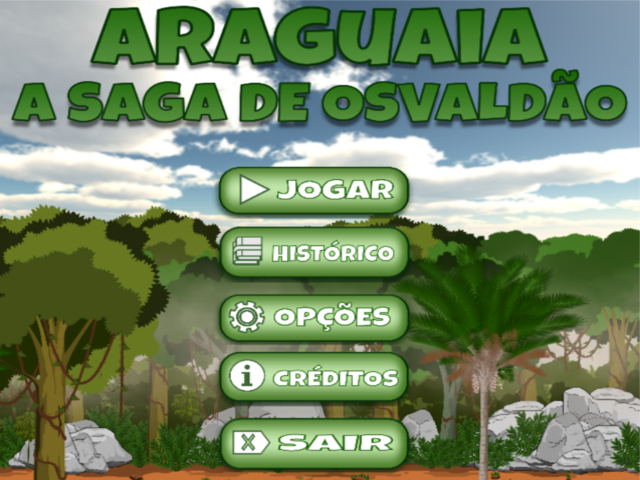
\includegraphics[width=0.56\textwidth]{figuras/menu_principal.png}
	\label{fig:menu-jogo}
	{\fonte{O Autor (2018)}}
\end{figure}

Ao clicar em ``HISTÓRICO", o jogador lerá um texto de $786$ palavras, com informações sobre a fundamentação histórica. Este texto é sucinto, e como é lido fora do ambiente do jogo não prejudica a sua jogabilidade. As outras informações não interativas são cinco \textit{cutscenes} -- uma \textit{3D}, que aparece ao jogador tocar em \textit{JOGAR} no menu principal da figura \ref{fig:menu-jogo}, que é muito importante para imergir o mesmo no enredo do jogo, e quatro pequenas \textit{cutscenes 2D}, em momentos importantes de transição entre as missões.

Além disso, o jogo conta com alguns elementos de interface gráfica comum em games, como \textit{HUD (Heads-up Display)}, que, em todas as missões, é composto pela barra de vidas do personagem, e um botão para acesso as opções de inventário para cada missão (figura \ref{fig:hud-jogo}).

\begin{figure}[H]
	\centering
	\caption{\textit{HUD} do Jogo}
	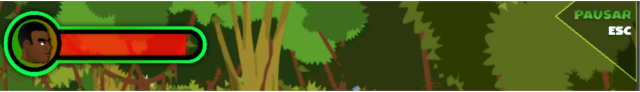
\includegraphics[width=0.7\textwidth]{figuras/hud_jogo.png}
	\label{fig:hud-jogo}
	{\fonte{O Autor (2018)}}
\end{figure}

As telas de inventário foram utilizadas em cada missão, para nortear o jogador quanto aos objetivos da missão, elas são acessíveis pelo botão ``PAUSAR", disponível na \textit{HUD} do game (conforme figura \ref{fig:hud-jogo}). Essa tela mostra o objetivo geral da missão, bem como os objetivos específicos que o jogador tem que cumprir. A figura \ref{fig:invent-miss1} apresenta o inventário da missão de capinar um terreno para fazer um campo de futebol, descrita na seção \ref{missao:const-campo}.

\begin{figure}[H]
	\centering
	\caption{Inventário da missão descrita na seção \ref{missao:const-campo}}
	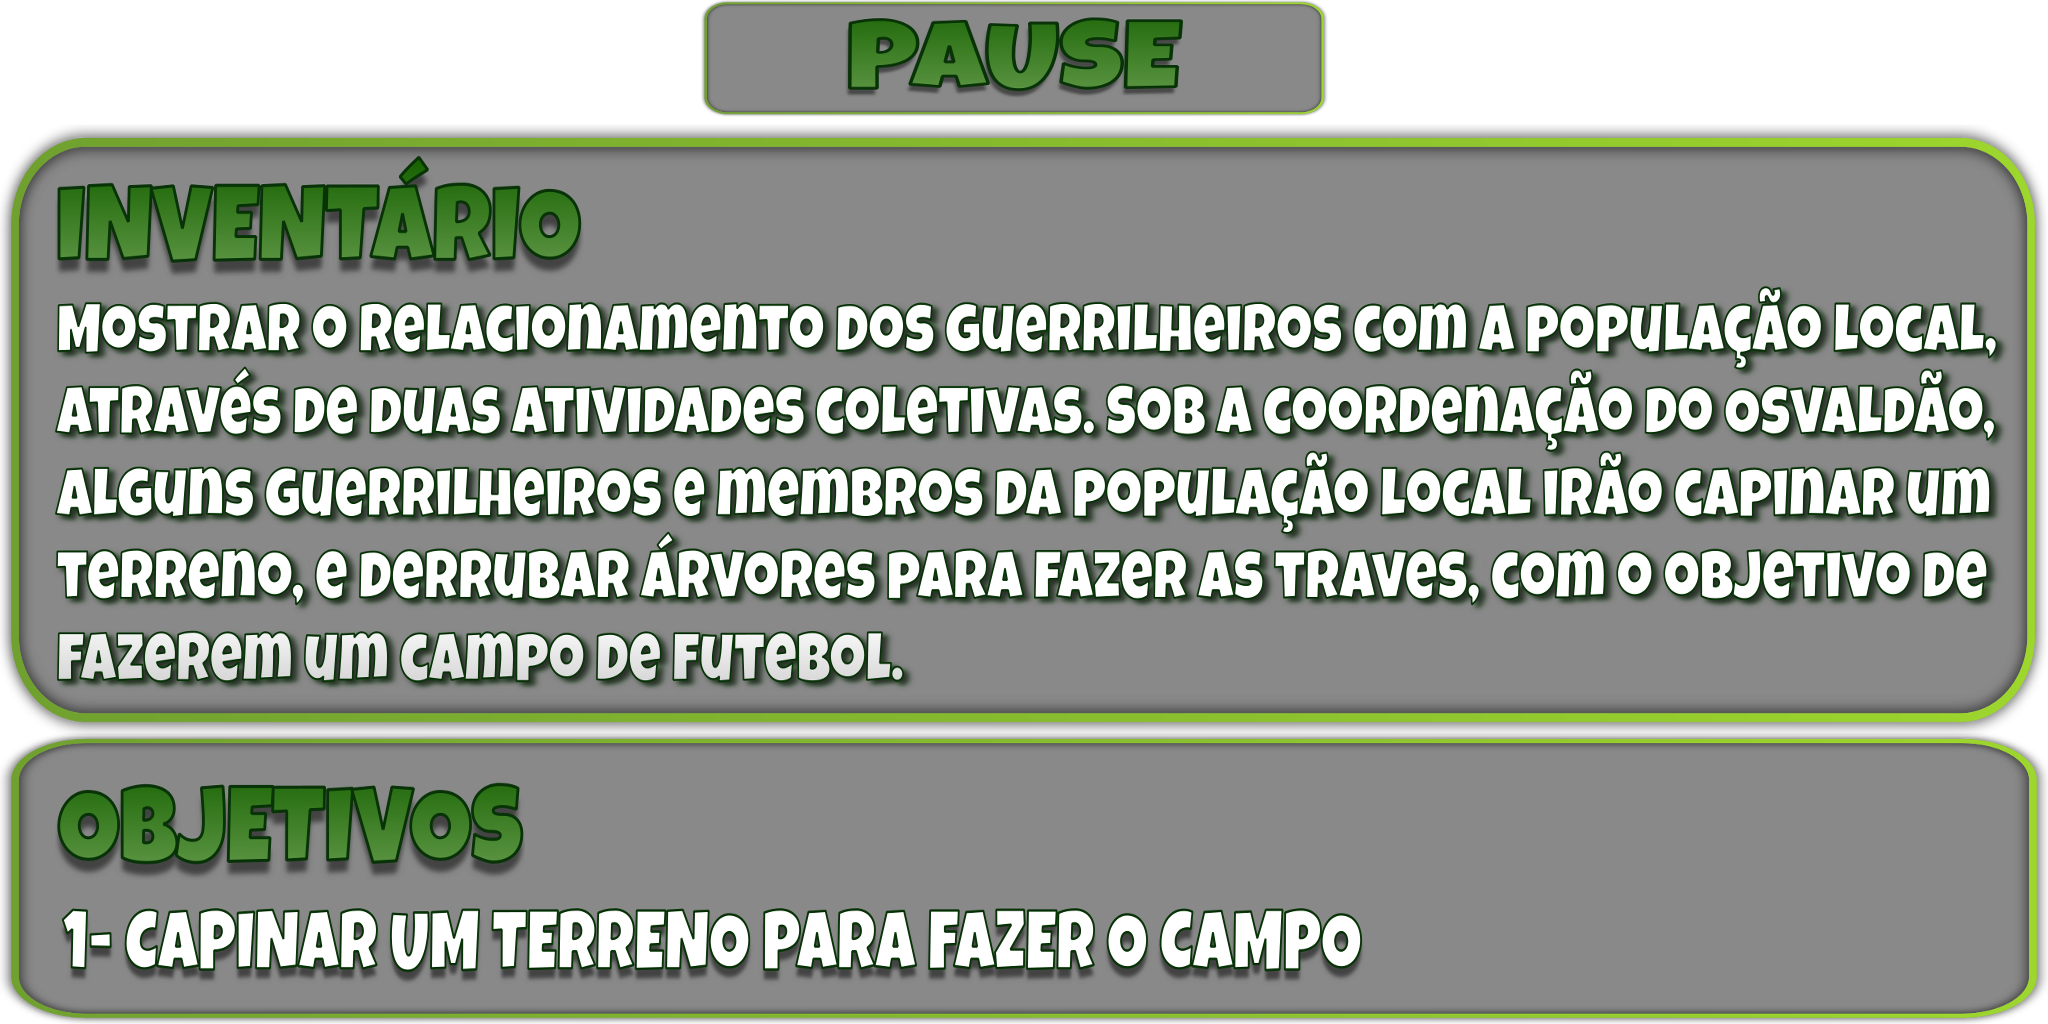
\includegraphics[width=0.7\textwidth]{figuras/inventario_miss1.png}
	\label{fig:invent-miss1}
	{\fonte{O Autor (2018)}}
\end{figure}

Quanto aos controles do jogo, basicamente contam com três botões principais (figura \ref{fig:botoes-jogo}), disparados por meio de eventos de \textit{touch screen}, comum em dispositivos móveis. O botão responsável por fazer o personagem caminhar tem funcionamento similar a uma alavanca (figura \ref{fig:botoes-jogo} – lado esquerdo). Desta maneira foi possível reduzir o número de botões na tela do \textit{smartphone} do usuário, facilitando a jogabilidade.

\begin{figure}[H]
	\centering
	\caption{Principais botões de controle do jogo}
	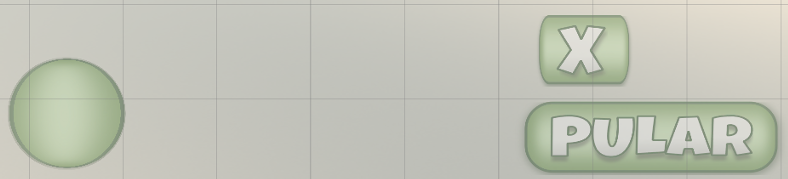
\includegraphics[width=0.7\textwidth]{figuras/botoes_jogo.png}
	\label{fig:botoes-jogo}
	{\fonte{O Autor (2018)}}
\end{figure}

\section{Implementação do Jogo}
\label{sec:implementacao}

Esta seção apresenta subsequentemente as quatro \textit{cutscenes} e as quatro missões implementadas pelo autor deste trabalho, as missões estão destacadas (negrito) na tabela \ref{tab:enrrotmis}. Também serão apresentados os objetivos, cenários e personagens de cada uma, bem como as ferramentas e técnicas utilizadas durante o processo.

\addtocontents{toc}{\protect\setcounter{tocdepth}{1}}
\subsection{\textit{Cutscene} inicial \textit{3D}}
\label{subsec:cutscene3D}

\addtocontents{toc}{\protect\setcounter{tocdepth}{1}}
\subsubsection{Descrição Geral}

Esta \textit{cutscene} tem como objetivo introduzir o jogador no jogo, fazendo com que este seja imerso no palco dos acontecimentos do passado, através de uma pequena narrativa no presente. Ela se passa na cidade de São Domingos do Araguaia, no tempo presente, em um local denominado ``Forte". Os personagens contidos nela são Osvaldão e um menino, um jovem curioso e observador a quem Osvaldão ``apresenta"\space suas experiências na Guerrilha.

\addtocontents{toc}{\protect\setcounter{tocdepth}{1}}
\subsubsection{Narrativa}

Fim de tarde. Pôr do sol. Um jovem observa, metros à frente, alguns meninos brincando no rio Araguaia, como ele tantas vezes fizera. Sem saber ao certo o porquê, sua mente parece querer decifrar algo escondido entre a margem e a correnteza do rio; entre o sorriso e a simetria dos movimentos realizados por aqueles meninos, que desafiam gravidade e medo saltitando de uma pilastra há muito deixada ali.

Há tempos, toda vez que observa o Araguaia, ou um dos resquícios de mata densa que ainda o cercam, o jovem parece ser tomado por uma espécie de saudade de algo que ele não consegue identificar ao certo, como se do leito de suas memórias fossem, a qualquer instante, emergir algo forte, vigoroso, visceral, como lembranças, guardadas em camadas mais profundas do que qualquer coisa que seus os seus olhos já puderam presenciar.

Ele pensava sobre isso, quando escuta um barulho perto de si. Ao olhar para o lado, vê que que um homem se aproxima do rio. Estranho não tê-lo notado até então, pensa, antes de ensaiar o retorno às suas viagens interiores.

\noindent
\textit{-- Sempre gostei dessa parte do rio. (Osvaldão)\\
-- Como? (Menino)\\
-- Gosto de como ele passa ao mesmo tempo sereno e caudaloso, como o tempo, como o tempo... (Osvaldão)\\
-- Faz tempo que o senhor vive aqui? (Menino)\\
-- Não poderia dizer que não faz... E sim, na época da Guerrilha também... (Osvaldão)\\
-- Como o senhor sabe que eu ia perguntar isso? (Menino)\\
-- Com o tempo, passamos a saber. (Osvaldão)\\
-- Diz que muitas coisas aconteceram aqui na época da Guerrilha. (Menino)\\
-- Muitas coisas, coisas demais... (Osvaldão)\\
-- Como assim? (Menino)\\
-- Coisas que os nossos olhos não foram criados para ver, mas que qual essas pedras no leito do rio, parecem sempre perseguir os homens, por onde quer que eles andem... (Osvaldão)\\
-- As vezes eu tenho alguns pensamentos, como se tivesse vivido naquela época, não sei se o senhor consegue me entender... Como se minha mente conseguisse ver mais do que está bem aqui diante dos meus olhos; mas, na verdade, não consigo ver é nada, nada além do que está de fato aqui. (Menino)\\
-- Se te interessa tanto ver, porque não tenta abrir um pouco mais a mente, ampliar mais o olhar, e sentir o que os outros sentidos são capazes de te dizer... (Osvaldão)\\
-- Como assim? (Menino)\\
-- Olhe comigo para as pedras, a água, a floresta, o sol, o horizonte... tente ver o que mais eles tem para lhe mostrar... Sinta o vento e o gosto de descoberta lhe acariciar a pele, a boca, lhe aguçar ainda mais os sentidos... (Osvaldão)}

Só agora o menino repara melhor no homem, então um pouco mais próximo de si. Um sujeito alto, negro, sorridente, que lhe provocou algo diferente, como se há muito já o conhecera. Não gasta, porém, muito tempo a analisa-lo, pois logo se absorve em percorrer o percurso indicado pelo outro, rumo ao sol, e ao ponto mais turvo das águas e da mata ali ao seu redor. Sua mente viaja, esvoaça por sobre o rio, a mata, o céu; plana sobre uma cachoeira qualquer do tempo, até voltar a si e desaguar num tempo e espaço de onde, logo sente, poderá encontrar a nascente das sensações que há muito lhe incomodam.

\addtocontents{toc}{\protect\setcounter{tocdepth}{1}}
\subsubsection{Ferramentas e Técnicas}

Para a implementação desta \textit{cutscene}, foi necessária uma coleta de dados, por meio do software \textit{Google Earth}\footnote{\url{https://www.google.com.br/earth/download/gep/agree.html}}, afim de obter uma imagem com a vista de topo do cenário. Além disto, utilizando uma câmera digital, foram feitas visitas ao ambiente para coleta de imagens e vídeos com o intuito de fazer uma extração arquitetônica mais detalhista da cena. A figura \ref{fig:forte-planta} apresenta a imagem extraída do \textit{Google Earth}.

As imagens coletadas durante as visitas ao ambiente real foram importantes para a texturização do cenário virtual, aumentando a sensação de realismo e imersão dele. O software \textit{Blender} fora empregado para a modelagem do ambiente, por meio da técnica de modelagem por imagem de referência, onde usa-se uma foto do modelo real, para a construção de sua versão virtual.

\begin{figure}[H]
	\centering
	\caption{Imagem extraída do \textit{Google Earth}}
	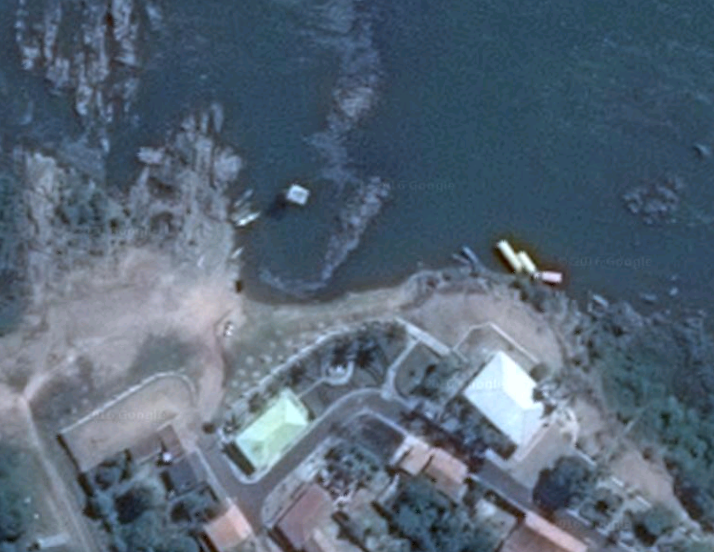
\includegraphics[width=0.7\textwidth]{figuras/forte_planta.png}
	\label{fig:forte-planta}
	{\fonte{O Autor (2018)}}
\end{figure}

Para a modelagem do personagem Osvaldão, foram utilizadas imagens extraídas da obra de \citeonline{bib:jofilly2008} como referência. Já o personagem menino foi modelado com base em um modelo genérico provido pela ferramenta de modelagem empregada (\textit{Makehuman}). O cenário \textit{3D} foi projetado a partir da imagem extraída do \textit{Google Earth}, que foi empregada como referência no software \textit{Blender}, dando uma base geral para a modelagem da cena. Assim, os modelos foram construídos, e através das fotos e vídeos capturados, fora possível a construção dos arredores do ambiente tridimensional, aumentando a sensação de realismo dele. A figura \ref{fig:forte-final} apresenta a \textit{cutscene 3D} finalizada com Osvaldão e o menino.

\begin{figure}[H]
	\centering
	\caption{Cenário da \textit{cutscene 3D}, Osvaldão e menino finalizados}
	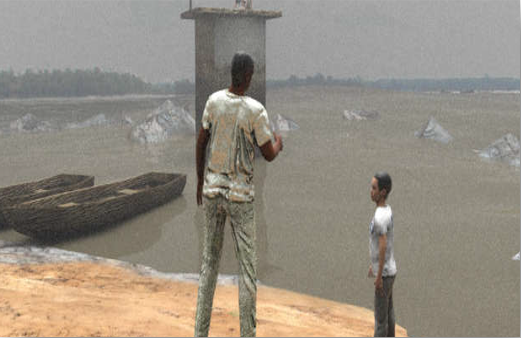
\includegraphics[width=0.73\textwidth]{figuras/osvaldo_final.png}
	\label{fig:forte-final}
	{\fonte{O Autor (2018)}}
\end{figure}

\addtocontents{toc}{\protect\setcounter{tocdepth}{1}}
\subsection{Missão -- Fundação do Destacamento $B$}
\label{missao:funddestacB}

\addtocontents{toc}{\protect\setcounter{tocdepth}{1}}
\subsubsection{Descrição Geral}

Esta missão apresenta ao jogador um fato histórico importante -- a criação de um primeiro barracão às margens do rio Gameleira, o local que, durante a Guerrilha, consolidou-se como o Destacamento $B$, tendo Osvaldão como o seu fundador e líder. Para realizar tal feito, o jogador deve controlar Osvaldão em um cenário cheio de obstáculos, representando um ambiente de mata fechada, com animais selvagens, pequenos riachos e armadilhas naturais, como troncos pontiagudos.

\addtocontents{toc}{\protect\setcounter{tocdepth}{1}}
\subsubsection{Roteiro}

As ações irão ocorrendo na medida em que o jogador vai movimentando Osvaldão da esquerda para a direita no cenário (Osvaldão aparece inicialmente no canto esquerdo da visão do jogador).

Em primeiro lugar, o jogador conduzirá Osvaldão tento como objetivo pular por cima de troncos pontiagudos (que irão aparecendo no meio do caminho) em meio à mata densa (estes troncos são frequentes no cenário). Após isto, Osvaldão tem que atravessar um pequeno riacho, lotado de piranhas. Para tanto, ele precisa pular sobre um tronco que flutua entre uma margem e outra do riacho. Posteriormente, Osvaldão precisa lutar com macacos quariba e porcões, podendo, nesta missão, atingi-los com um facão -- ``o facão era usado para tudo na floresta"\space\cite{bib:jofilly2008}. A figura \ref{fig:osvaldo-animais} apresenta o personagem enfrentando os animais da mata.

\begin{figure}[H]
	\centering
	\caption{Osvaldão lutando contra os animais da floresta}
	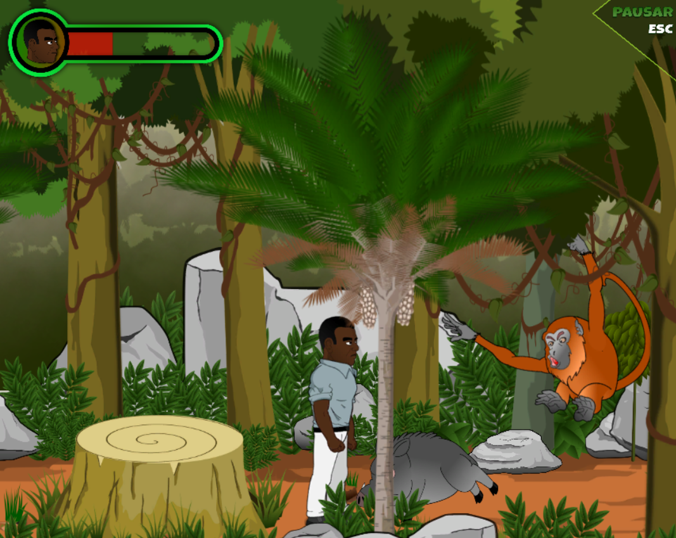
\includegraphics[width=0.57\textwidth]{figuras/osvaldo_animais_fase2.png}
	\label{fig:osvaldo-animais}
	{\fonte{O Autor (2018)}}
\end{figure}

Depois de lutar contra os animais da floresta, Osvaldão deve atravessar o rio Gameleira, lotado de piranhas, pulando sobre vários troncos que aparecem flutuando sobre o rio. Após atravessar o rio (figura \ref{fig:osvaldo-gameleira}), o personagem tem de tocar em um ícone de casa, finalizando a missão, e recebendo os primeiros guerrilheiros.

\begin{figure}[H]
	\centering
	\caption{Osvaldão atravessando o rio Gameleira}
	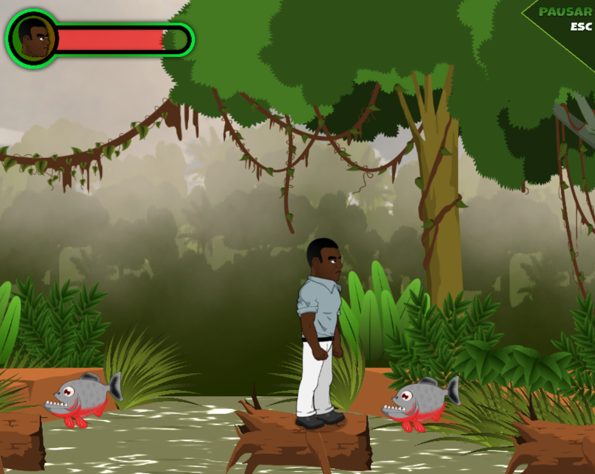
\includegraphics[width=0.56\textwidth]{figuras/osvaldo_gameleira_fase2.png}
	\label{fig:osvaldo-gameleira}
	{\fonte{O Autor (2018)}}
\end{figure}

\addtocontents{toc}{\protect\setcounter{tocdepth}{1}}
\subsubsection{Ferramentas e Técnicas}

Para a criação desta missão, o software \textit{Inkscape} foi utilizado para o desenho de todos os elementos do cenário \textit{2D} (alguns podem ser vistos na figura \ref{fig:elementos-2d}). Após esta etapa, os elementos foram exportados para o motor de jogos \textit{Unity} e organizados para formar a cena, alguns trechos da cena foram apresentados nas figuras \ref{fig:osvaldo-animais} e \ref{fig:osvaldo-gameleira}. A arte \textit{2D} dos cenários foi desenvolvida por bolsistas de extensão e voluntários, membros do projeto. Com a cena formada, o próximo passo foi a criação das regras definidas para a missão, por meio de \textit{scripts} em linguagem de programação C$\sharp$, também na \textit{Unity}.

\begin{figure}[H]
	\centering
	\caption{Alguns elementos dos cenários \textit{2D}}
	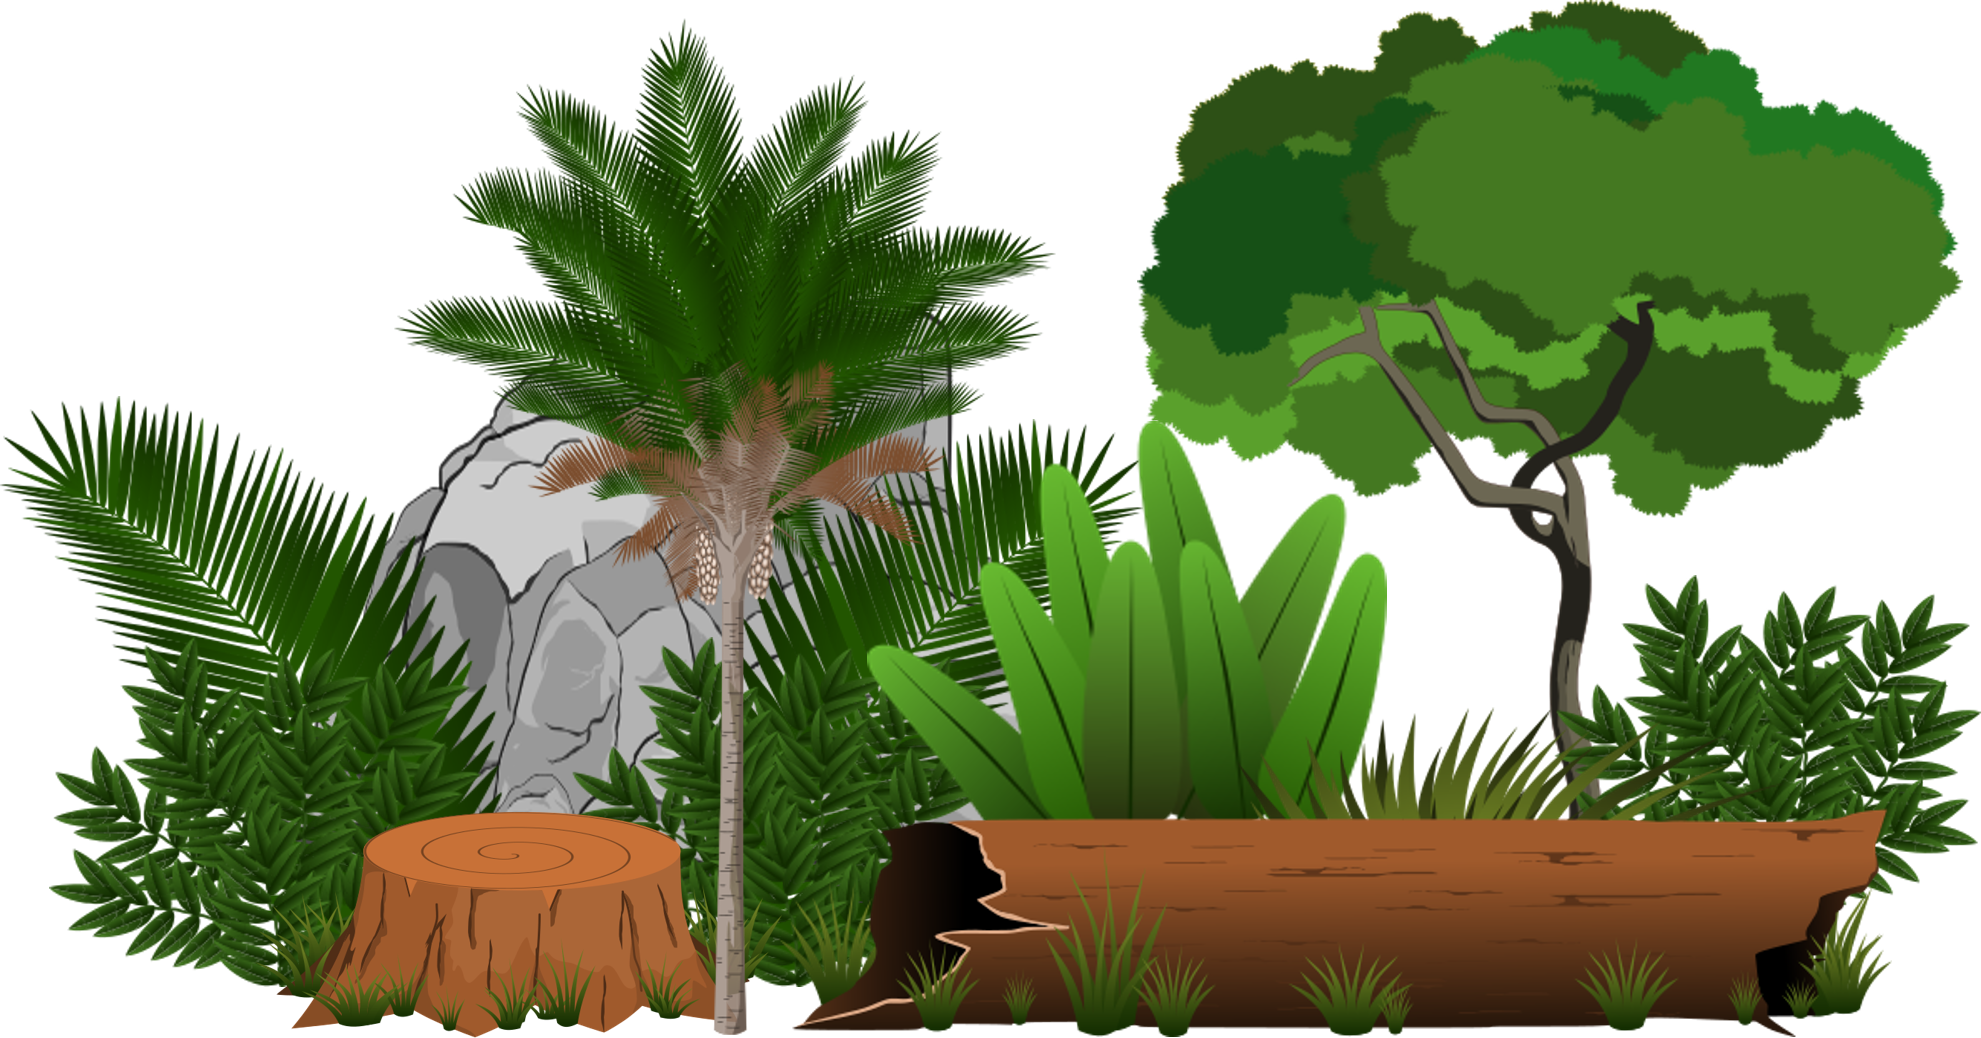
\includegraphics[width=0.75\textwidth]{figuras/elementos_2d.png}
	\label{fig:elementos-2d}
	{\fonte{O Autor (2018)}}
\end{figure}

\addtocontents{toc}{\protect\setcounter{tocdepth}{1}}
\subsection{\textit{Cutscene} -- Construção do Barracão do Destacamento B}

\addtocontents{toc}{\protect\setcounter{tocdepth}{1}}
\subsubsection{Descrição Geral}

O palco dos acontecimentos desta \textit{cutscene} é a região do ``Bico do Papagaio"\space -- confluência dos estados do Pará (Sul), Maranhão (Sul) e Goiás (atual norte do Tocantins). Região marcada por rios, floresta densa, serras, cavernas. Ela apresenta ao jogador o momento em que Osvaldão constrói o primeiro barracão do Destacamento $B$ e recepciona os primeiros guerrilheiros -- José Genoíno e Glênio Sá, essa é uma cena histórica importante, Osvaldão, que chegou  na região da guerrilha antes de todos os outros guerrilheiros para reconhecimento do local, recebe os seus primeiros companheiros de luta, no futuro Destacamento $B$, do qual ele se tornaria o comandante. Esta \textit{cutscene} também é uma continuação da missão descrita na seção \ref{missao:funddestacB}.

\addtocontents{toc}{\protect\setcounter{tocdepth}{1}}
\subsubsection{Narrativa}

Esta \textit{cutscene} inicia com Osvaldão se movendo da esquerda para a direita na cena, enquanto o seguinte texto vai sendo apresentado ao jogador:

\noindent
\textit{Depois de enfrentar os desafios da adaptação no Araguaia, Osvaldão assume uma nova missão: receber os novos companheiros Glênio, Genuíno... e Ajudá-los a se instalarem nas proximidades do rio Gameleira.\\
Será um grande desafio para quem acabou de chegar e ainda não conhece nada do terreno e de como sobreviver na floresta.\\
Osvaldão passa a orientá-los no trabalho da lavoura, na caça, pesca, no contato com a população local e nos treinamentos militares no interior da floresta.\\
O futuro do Destacamento $B$ começa a se formar, muita coisa ainda está por vir...}

Após a apresentação deste texto, a \textit{cutscene} é encerrada, deixando um ar de dúvida no jogador, fazendo com que ele tenha curiosidade em continuar jogando e descobrindo o que virá pela frente.

\addtocontents{toc}{\protect\setcounter{tocdepth}{1}}
\subsubsection{Ferramentas e Técnicas}

Para a criação desta \textit{cutscene}, foram utilizados modelos de vegetação, animais, construções e humanoides (personagens Genuíno e Glênio) em \textit{2D} concebidos pelos artistas da equipe do projeto com a ferramenta \textit{Inkscape}, e com base em imagens de referência capturadas durante as viagens aos locais onde ocorreu a Guerrilha. Estes modelos foram transportados para a \textit{Unity}, dando forma à cena. Posteriormente, fora produzido um vídeo do personagem Osvaldão caminhando na cena em direção ao barracão construído, onde os personagens Genuíno e Glênio o aguardam. A figura \ref{fig:cutscene1-fase1} mostra o momento do encontro entre estes personagens e Osvaldão.

\begin{figure}[H]
	\centering
	\caption{Trecho final da \textit{cutscene}, mostrando Osvaldão e seus novos companheiros no futuro Destacamento $B$}
	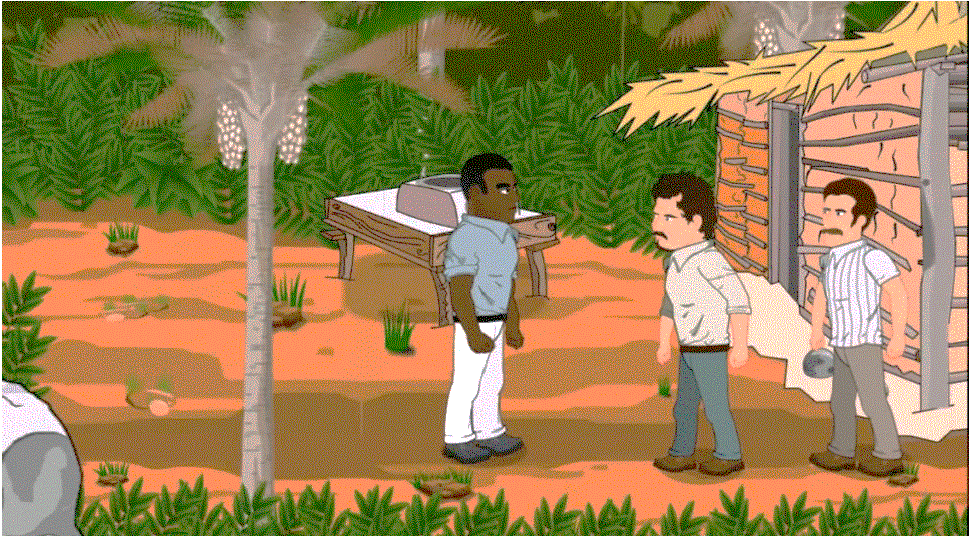
\includegraphics[width=0.7\textwidth]{figuras/cutscene1_fase1.png}
	\label{fig:cutscene1-fase1}
	{\fonte{O Autor (2018)}}
\end{figure}

\addtocontents{toc}{\protect\setcounter{tocdepth}{1}}
\subsection{Missão -- Expulsão do Grileiro (Pedro Mineiro)}
\label{missao:expgrileiro}

\addtocontents{toc}{\protect\setcounter{tocdepth}{1}}
\subsubsection{Descrição Geral}

O objetivo desta missão é apresentar ao jogador um episódio histórico pouco conhecido no âmbito da Guerrilha: a expulsão de um grileiro conhecido como Pedro Mineiro, feita por Osvaldão, no momento em que este apresentava a mata para os seus companheiros -- Maria Dina, José Genuíno, Glênio Sá e André Grabois. De repente, eles avistam o grileiro Pedro Mineiro e seus capangas oprimindo uma família de camponeses. Osvaldão troca tiros com eles, e consegue expulsá-los. Após a família de camponeses agradecer Osvaldão, este continua o passeio com seus amigos.

\addtocontents{toc}{\protect\setcounter{tocdepth}{1}}
\subsubsection{Roteiro}

Osvaldão, desta vez acompanhado por seus recém-chegados colegas Glênio, Genuíno, Maria Dina e André Grabóis, inicia a missão tendo que lutar contra os animais da floresta (porcões, macacos guariba e piranhas). Depois de avançar no confronto contra os animais, Osvaldão e sua equipe avistam o grileiro Pedro mineiro e seus capangas oprimindo uma família de camponeses. Osvaldão deve trocar tiros com o bando de Pedro Mineiro, para expulsá-los. A figura \ref{fig:osvaldo-grileiro} apresenta Osvaldão trocando tiros com Pedro Mineiro.

\begin{figure}[H]
	\centering
	\caption{Osvaldão trocando tiros com Pedro Mineiro}
	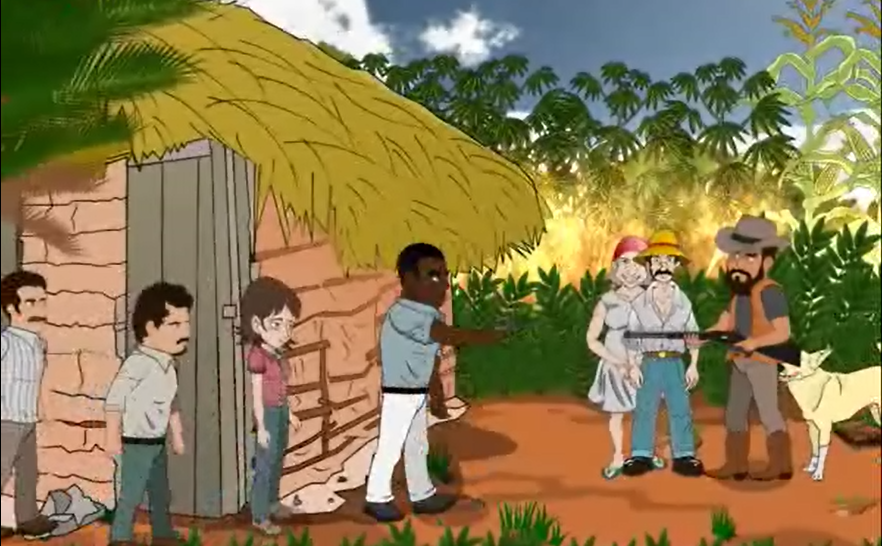
\includegraphics[width=0.56\textwidth]{figuras/osvaldo_grileiro_fase2.png}
	\label{fig:osvaldo-grileiro}
	{\fonte{O Autor (2018)}}
\end{figure}

Após a expulsão de Pedro Mineiro e seus capangas, é exibida uma \textit{cutscene} que inicia com Pedro Mineiro jogando uma maldição em Osvaldão, e finaliza com um passeio deste e seus companheiros pela floresta, sendo seguidos pelo pássaro curió.

\addtocontents{toc}{\protect\setcounter{tocdepth}{1}}
\subsubsection{Ferramentas e Técnicas}

Para esta missão, o software \textit{Inkscape} foi utilizado para o desenho de todos os elementos do cenário \textit{2D} (alguns podem ser vistos na figura \ref{fig:elementos-2d}), bem como dos personagens (Glênio, Genuíno, Maria Dina e André Grabóis). Após esta etapa, os elementos foram exportados para o motor de jogos \textit{Unity} e organizados para formar a cena, alguns trechos da cena podem ser vistos nas figuras \ref{fig:osvaldo-grileiro} e \ref{fig:osvaldo_equipe_fase2}. A arte \textit{2D} dos cenários e os personagens foram desenvolvidos por bolsistas de extensão e voluntários, membros do projeto. Para o desenvolvimento dos personagens, foram utilizadas referências de fotos reais deles, extraídas das bibliografias \citeonline{bib:glenio1990}, \citeonline{bib:jofilly2008} e \citeonline{bib:silva2012}. Com a cena formada, o próximo passo foi a criação das regras definidas para a missão, por meio de \textit{scripts} em linguagem de programação C$\sharp$, também usando a \textit{Unity}.

\begin{figure}[H]
	\centering
	\caption{Osvaldão e seus companheiros enfrentando os animais na mata}
	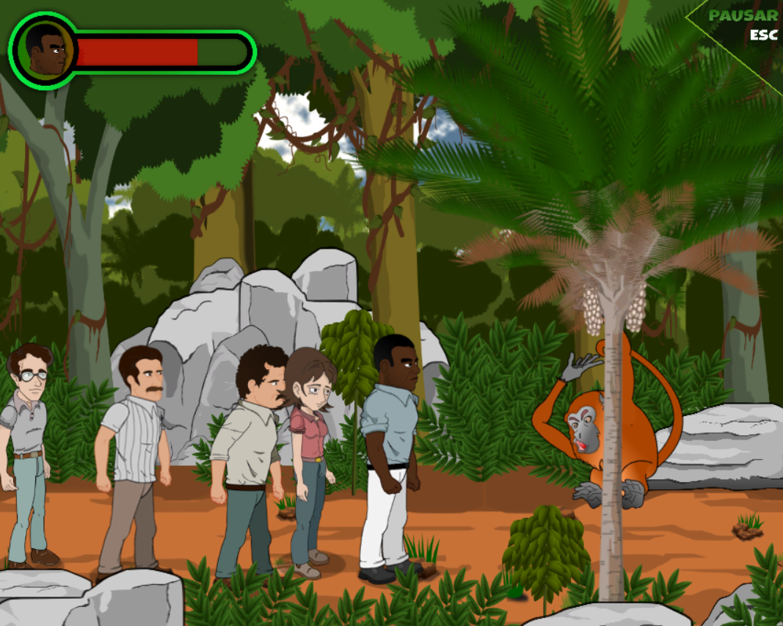
\includegraphics[width=0.6\textwidth]{figuras/osvaldo_equipe_fase2.png}
	\label{fig:osvaldo_equipe_fase2}
	{\fonte{O Autor (2018)}}
\end{figure}

\addtocontents{toc}{\protect\setcounter{tocdepth}{1}}
\subsection{\textit{Cutscene} -- Lançamento da praga do Capa verde}

\addtocontents{toc}{\protect\setcounter{tocdepth}{1}}
\subsubsection{Descrição Geral}

Esta \textit{cutscene} objetiva apresentar o lançamento da praga do ``Capa verde", realizada pelo grileiro temido na região, conhecido como Pedro Mineiro, após Osvaldão expulsá-lo com seus capangas das terras de uma família de camponeses (missão descrita na seção \ref{missao:expgrileiro}).

\addtocontents{toc}{\protect\setcounter{tocdepth}{1}}
\subsubsection{Narrativa}

A \textit{cutscene} inicia logo após Osvaldão expulsar Pedro mineiro e seus capangas (retratado na missão descrita na seção \ref{missao:expgrileiro}). Nela, o personagem principal e seus companheiros movimentam-se da esquerda para a direita da tela. E, ao chegar em certo ponto do cenário, eles deparam-se com Pedro Mineiro, desta vez, sozinho. Então, o grileiro faz o seguinte discurso:

\noindent
\textit{Num comemorem demais não. Cês vão ver. Tá chegando o dia que o Padim ciço falô, o tempo do capa verda. O tempo da guerra tá chegando, o Araguaia vai banzeirar numa metade e na outra vai ferver. E bem ali no meio do redemuinho vão tá vocês, vocês e o Capa verde.}

Após fazer o diálogo, Pedro Mineiro some no meio da mata densa. Osvaldão e seus companheiros continuam o passeio. Sendo acompanhados misteriosamente por um pássaro curió.

\addtocontents{toc}{\protect\setcounter{tocdepth}{1}}
\subsubsection{Ferramentas e Técnicas}

Nesta \textit{cutscene}, foram utilizados modelos de vegetação, animais e humanoides (personagens Osvaldão, Genuíno, Glênio, Dina, Grabois e Pedro Mineiro) em \textit{2D} concebidos pelos artistas da equipe do projeto com a ferramenta \textit{Inkscape}, e com base em imagens de referência capturadas durante as viagens aos locais onde ocorreu a Guerrilha. Estes modelos foram transportados para a \textit{Unity}, dando forma à cena. Posteriormente, fora produzido um vídeo do personagem Osvaldão com os seus companheiros (Genuíno, Glênio, Dina e Grabois) caminhando para a frente, quando são deparados com a presença do grileiro. A figura \ref{fig:cutscene2-fase1} mostra o momento em que Pedro Mineiro lança a praga do Capa verde em Osvaldão e seus companheiros.

\begin{figure}[H]
	\centering
	\caption{Trecho da \textit{cutscene}, onde Pedro Mineiro lança uma maldição nos guerrilheiros}
	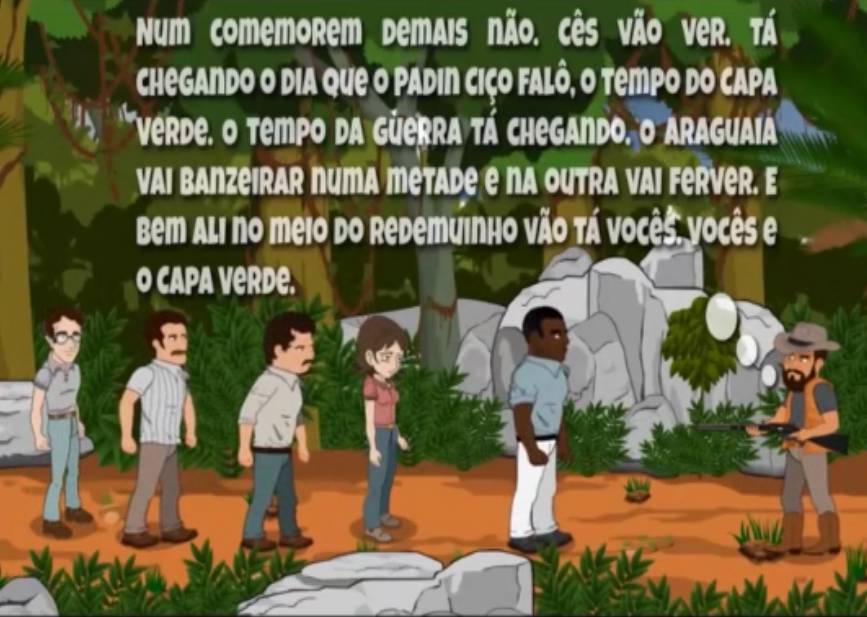
\includegraphics[width=0.6\textwidth]{figuras/cutscene2_fase1.png}
	\label{fig:cutscene2-fase1}
	{\fonte{O Autor (2018)}}
\end{figure}

\begin{figure}[H]
	\centering
	\caption{Trecho final da \textit{cutscene}, onde Osvaldão e seus companheiros continuam o passeio após Pedro Mineiro lançar a maldição}
	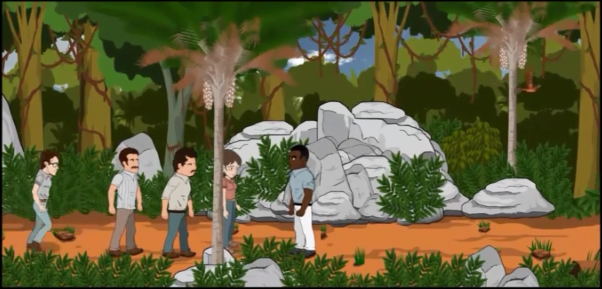
\includegraphics[width=0.65\textwidth]{figuras/cutscene21_fase1.png}
	\label{fig:cutscene21-fase1}
	{\fonte{O Autor (2018)}}
\end{figure}

\addtocontents{toc}{\protect\setcounter{tocdepth}{1}}
\subsection{Missão -- Construção do Campo de Futebol}
\label{missao:const-campo}

\addtocontents{toc}{\protect\setcounter{tocdepth}{1}}
\subsubsection{Descrição Geral}

Esta missão apresenta uma atividade realizada pelos guerrilheiros, juntamente com a população local camponesa: a construção de um campo de futebol. A missão ocorre em dois momentos. O primeiro onde, Osvaldão, um morador e Genuíno fazem um mutirão para limpar um terreno onde será construído o campo. O segundo onde, o morador entra na mata para cortar árvores com o machado, para a construção das traves. 

\addtocontents{toc}{\protect\setcounter{tocdepth}{1}}
\subsubsection{Roteiro}

Inicia com o jogador controlando Osvaldão, junto com um cachorro (em \citeonline{bib:jofilly2008} é relatado que ele tinha um cachorro) ao seu lado, em uma vila próxima ao Destacamento $B$. Osvaldão caminha enquanto acena para as pessoas da vila. Em seguida, aparece um obstáculo -- capinar um terreno para a construção de um campo de futebol (figura \ref{fig:osvaldo_capinando}). Inicialmente o jogador controla o Osvaldão, e ao fundo aparece o guerrilheiro Genuíno e um morador realizando o mesmo trabalho. Quando o jogador vencer algumas etapas (limpar uma parte do terreno, com o perigo das serpentes escondidas em meio a vegetação), um dos populares que está ao fundo passa a ser controlado pelo jogador, e o Osvaldão e o cachorro passam a agir livremente. O personagem que o jogador controla, de vez em quando muda, podendo ser o guerrilheiro ou um morador, e sempre aparece o Osvaldão trabalhando junto com guerrilheiros e populares. Depois de vencer a etapa da capinação, começa a etapa de corte de madeira (figura \ref{fig:morador_tronco}). O processo é semelhante ao anterior. O personagem morador é controlado pelo jogador com um machado na mão, que adentra na mata, enfrentando obstáculos como serpentes, ribanceiras e porcões para cortar um tronco de árvore, usado para a construção das traves.

\begin{figure}[H]
	\centering
	\caption{Osvaldão, morador e Genuíno capinando um terreno para fazer o campo}
	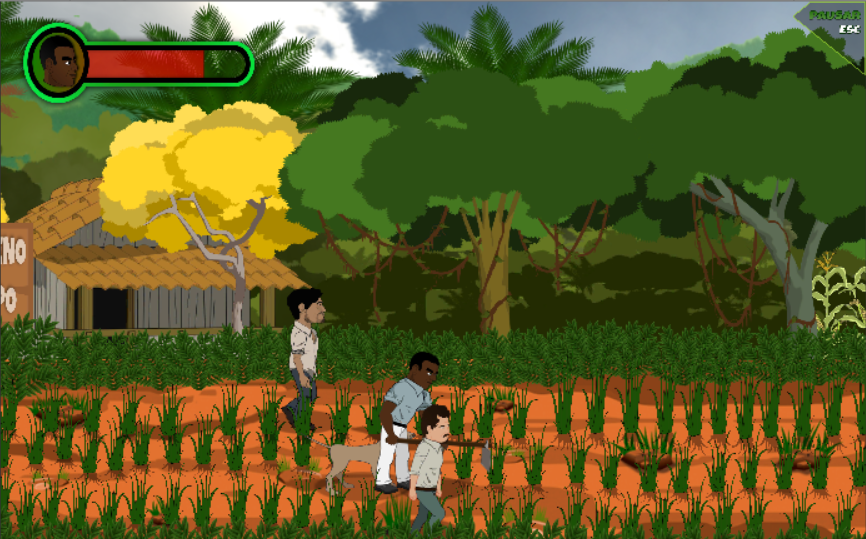
\includegraphics[width=0.62\textwidth]{figuras/osvaldo_capinando.png}
	\label{fig:osvaldo_capinando}
	{\fonte{O Autor (2018)}}
\end{figure}

\begin{figure}[H]
	\centering
	\caption{Morador cortando tronco para as traves}
	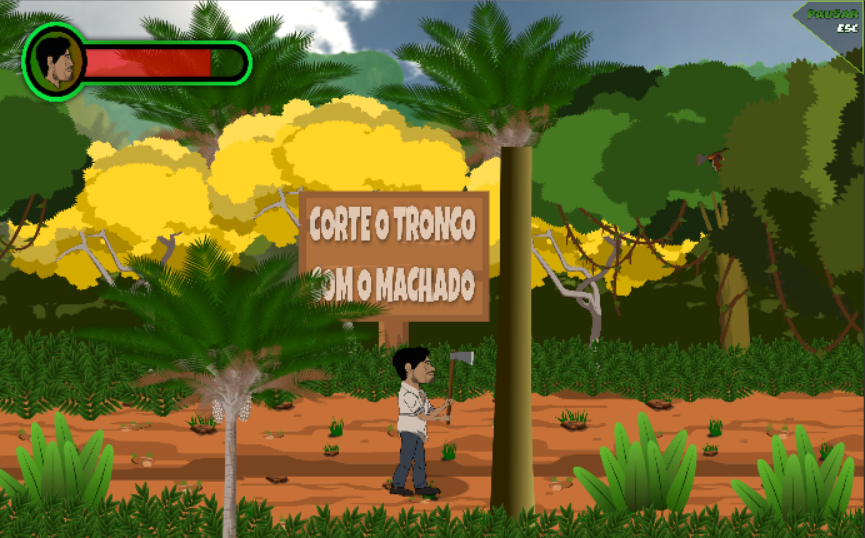
\includegraphics[width=0.62\textwidth]{figuras/morador_tronco.png}
	\label{fig:morador_tronco}
	{\fonte{O Autor (2018)}}
\end{figure}

\addtocontents{toc}{\protect\setcounter{tocdepth}{1}}
\subsubsection{Ferramentas e Técnicas}

Para a criação desta missão, o software \textit{Inkscape} foi utilizado para o desenho de todos os elementos dos cenários (alguns podem ser vistos na figura \ref{fig:elementos-2d}). Após esta etapa, os elementos foram exportados para o motor de jogos \textit{Unity} e organizados para formar as cenas (cena da vila e do corte de madeira), apresentadas nas figuras \ref{fig:osvaldo_capinando} e \ref{fig:morador_tronco}, respectivamente. A arte \textit{2D} dos cenários foi desenvolvida por bolsistas de extensão e voluntários, membros do projeto. Com a cena formada, o próximo passo foi a criação das regras definidas para a missão, por meio de \textit{scripts} em linguagem de programação C$\sharp$, também na \textit{Unity}.

\addtocontents{toc}{\protect\setcounter{tocdepth}{1}}
\subsection{\textit{Cutscene} -- Guerrilheiros e moradores inaugurando o campo de futebol construído}

\addtocontents{toc}{\protect\setcounter{tocdepth}{1}}
\subsubsection{Descrição Geral}

Após o êxito na construção do campo de futebol (relatada na missão descrita na seção \ref{missao:const-campo}), Osvaldão, guerrilheiros e moradores inauguram o campo, em um momento de descontração, jogando uma partida de futebol.

\addtocontents{toc}{\protect\setcounter{tocdepth}{1}}
\subsubsection{Narrativa}

Osvaldão inicia no canto esquerdo do campo de futebol, e a bola de futebol inicia no meio do campo. Osvaldão vai de encontro a bola, e a partida começa. Enquanto isso, o texto a seguir é passado na tela do jogo:

\noindent
\textit{Guerrilheiros e camponeses batem uma pelada após construírem o campo de futebol.\\
Os camponeses chamam os guerrilheiros de Paulistas. Não conhecem, ainda, seus objetivos na região.}

Após a passagem deste texto, Osvaldão para próximo à trave direita do campo de futebol. Finalizando a \textit{cutscene}.

\addtocontents{toc}{\protect\setcounter{tocdepth}{1}}
\subsubsection{Ferramentas e Técnicas}

Nesta \textit{cutscene}, foram utilizados modelos de vegetação, animais e humanoides em \textit{2D} concebidos pelos artistas da equipe do projeto com a ferramenta \textit{Inkscape}, e com base em imagens de referência capturadas durante as viagens aos locais onde ocorreu a Guerrilha. Estes modelos foram transportados para a \textit{Unity}, dando forma à cena. Posteriormente, fora produzido um vídeo dos personagens se movimentando no campo. A figura \ref{fig:osvaldao_campo} mostra o momento em que Osvaldão inícia a partida de futebol. Já a figura \ref{fig:osvaldao_campo}, mostra o momento em que Osvaldão finaliza a partida.

\begin{figure}[H]
	\centering
	\caption{Osvaldão iniciando a partida de futebol no campo recém criado}
	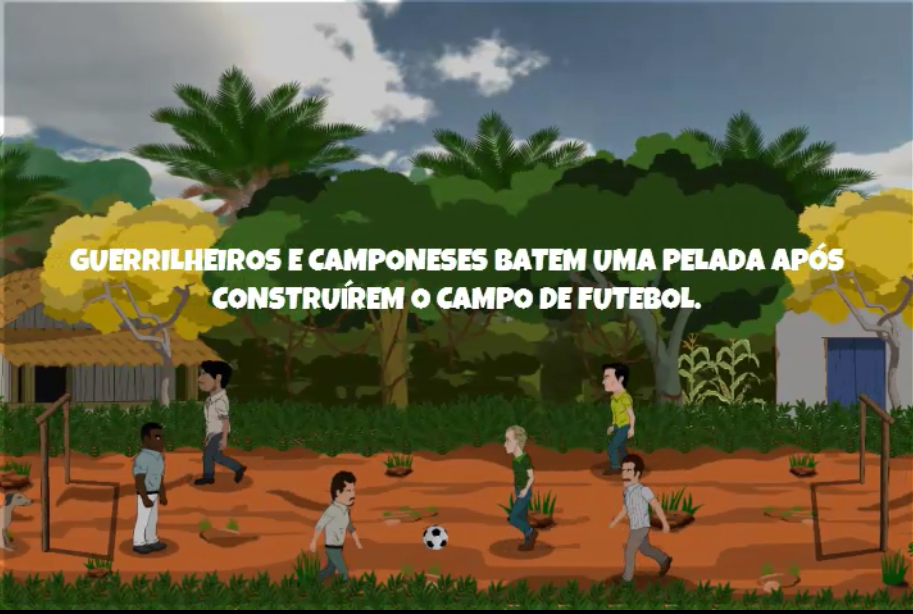
\includegraphics[width=0.62\textwidth]{figuras/osvaldao_campo.png}
	\label{fig:osvaldao_campo}
	{\fonte{O Autor (2018)}}
\end{figure}

\begin{figure}[H]
	\centering
	\caption{Osvaldão finalizando a partida de futebol no campo recém criado}
	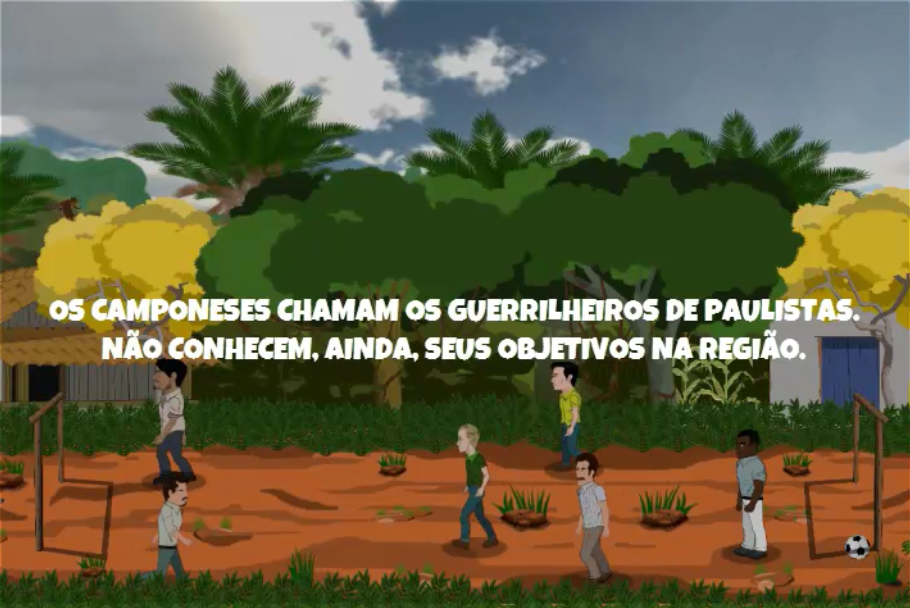
\includegraphics[width=0.62\textwidth]{figuras/osvaldao_campo_2.png}
	\label{fig:osvaldao_campo_2}
	{\fonte{O Autor (2018)}}
\end{figure}

\addtocontents{toc}{\protect\setcounter{tocdepth}{1}}
\subsection{Missão -- Combate entre os Militares e Guerrilheiros}

\addtocontents{toc}{\protect\setcounter{tocdepth}{1}}
\subsubsection{Descrição Geral}

Esta missão tem como objetivo mostrar um episódio ocorrido na Guerrilha, que resultou na morte de um militar ás margens do rio Gameleira, conhecido como Cabo Rosa, após uma intensa troca de tiros entre ele e Osvaldão. A missão é dividida em dois momentos. No primeiro, o jogador controla o Tenente Nélio, em um barco, com mais três militares e um guia, objetivando atravessar o rio Araguaia para adentrar na mata fechada. Em um segundo momento, o jogador controla Osvaldão, acompanhado do guerrilheiro Bergson, que caminham na mata para esconder suprimentos e armadilhas. Perto do rio Gameleira, eles acabam se deparando com os militares, havendo uma intensa troca de tiros, acarretando na morte de um dos militares.

\addtocontents{toc}{\protect\setcounter{tocdepth}{1}}
\subsubsection{Roteiro}

A missão fora dividida em dois momentos. O primeiro inicia com o jogador controlando o Tenente Nélio, em um barco, objetivando a travessia do rio Araguaia, conforme figura \ref{fig:nelio_barco}. Nessa parte, Nélio deve esquivar-se dos ataques de piranhas ou bater nelas com um facão para sobreviver em cima da embarcação. Este momento finaliza com a travessia do barco e a descida do Nélio em terra firme. Já segundo inicia com o jogador controlando Osvaldão, acompanhado do guerrilheiro Bergson, na mata densa. Sendo vigiada por militares. O jogador deve controlar Osvaldão, de modo a vencer os perigos impostos na fase (serpentes, helicópteros disparando bombas e etc). Essa fase termina quando Osvaldão chega no rio Gameleira -- local onde ele e Bergson se encontram com os militares que chegaram de barco. Ai, ocorre uma troca de tiros entre Osvaldão (portando uma espingarda) e os demais militares, acarretando na morte do militar conhecido como Cabo Rosa (portando uma metralhadora), conforme a figura \ref{fig:osvaldao_tiros_cabo}, após ser atingido por Osvaldão.

\begin{figure}[H]
	\centering
	\caption{Tenente Nélio e demais militares atravessando o rio Araguaia}
	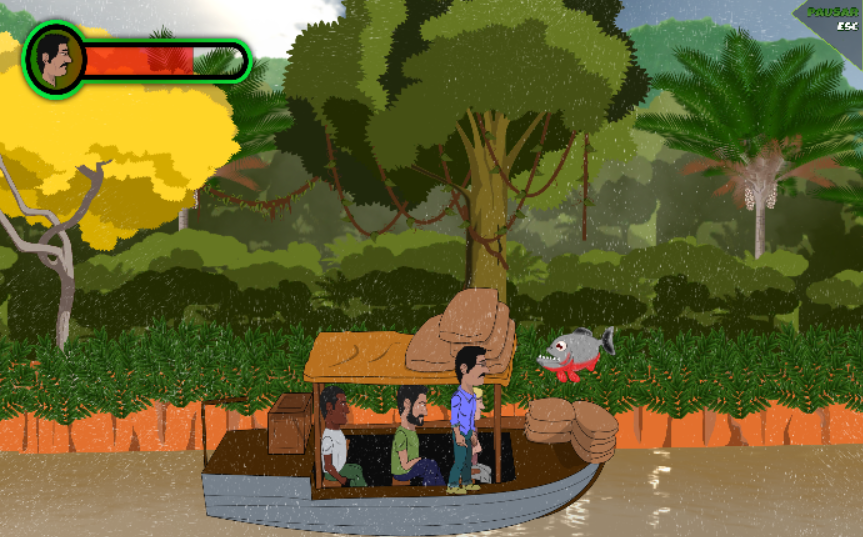
\includegraphics[width=0.62\textwidth]{figuras/nelio_barco.png}
	\label{fig:nelio_barco}
	{\fonte{O Autor (2018)}}
\end{figure}

\begin{figure}[H]
	\centering
	\caption{Osvaldão trocando tiros com o Cabo Rosa}
	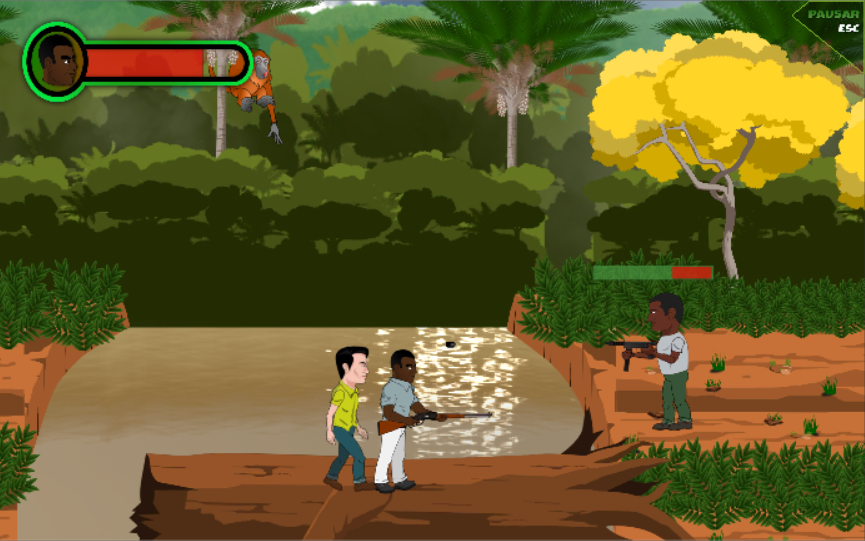
\includegraphics[width=0.62\textwidth]{figuras/osvaldao_tiros_cabo.png}
	\label{fig:osvaldao_tiros_cabo}
	{\fonte{O Autor (2018)}}
\end{figure}

\addtocontents{toc}{\protect\setcounter{tocdepth}{1}}
\subsubsection{Ferramentas e Técnicas}

Para desta missão, o software \textit{Inkscape} foi utilizado para o desenho de todos os elementos do cenário (alguns podem ser vistos na figura \ref{fig:elementos-2d}). Após esta etapa, os elementos foram exportados para o motor de jogos \textit{Unity} e organizados para formar a cena, apresentada nas figuras \ref{fig:nelio_barco} e \ref{fig:osvaldao_tiros_cabo}. A arte \textit{2D} dos cenários foi desenvolvida por bolsistas de extensão e voluntários, membros do projeto. Com a cena formada, o próximo passo foi a criação das regras definidas para a missão, por meio de \textit{scripts} em linguagem de programação C$\sharp$, também na \textit{Unity}.

\section{Avaliação do Jogo}
\label{sec:avaliacao}

Seguindo o modelo de desenvolvimento utilizado pela equipe, descrito na seção \ref{sec:desenvolvimento}. O próximo passo foi dado com a avaliação do jogo, dividida em: avaliação técnica, avaliação pedagógica e avaliação com alunos.

A avaliação técnica foi realizada por toda a equipe do projeto -- após cada integração e reunião de acompanhamento -- por meio de testes unitários para verificação de erros e análise da jogabilidade, desempenho e compatibilidade entre diversos dispositivos e versões do sistema operacional \textit{Android}.

A avaliação pedagógica foi de responsabilidade de um dos coordenadores do projeto, que é professor de história, juntamente com outro professor de história de uma escola do município de Marabá-PA. Esta avaliação teve o intuito de checar a adequação do jogo educativo ao seu objetivo pedagógico e validá-lo como ferramenta auxiliar no processo de ensino/aprendizagem sobre a Guerrilha do Araguaia na disciplina de História das escolas do ensino médio.

Até o momento, foi realizada uma apresentação do jogo para alguns alunos de uma das escolas do ensino médio de Marabá-PA, com o objetivo de receber o \textit{feedback} deles. Antes da apresentação do jogo, os alunos participaram de uma palestra com o objetivo de apresentar o processo de produção de um jogo, apresentada na figura \ref{fig:palestra-jogos}, além de introduzir os produtos digitais produzidos para auxilio ao ensino de história. Durante a apresentação, os alunos mostraram boa aceitação do jogo quanto a aspectos de interface e jogabilidade. A figura \ref{fig:palestra-jogos} mostra um aluno testando o jogo. Futuramente, mais testes serão realizados em várias escolas do município, objetivando tabular dados estatísticos que revelem a eficiência e eficácia do jogo como ferramenta de aprendizado.

\begin{figure}[H]
	\centering
	\caption{Palestra sobre o processo de produção de um jogo}
	\includegraphics[width=0.7\textwidth]{figuras/workshop_alunos.jpg}
	\label{fig:palestra-jogos}
	{\fonte{O Autor (2018)}}
\end{figure}

\begin{figure}[H]
	\centering
	\caption{Aluno testando o jogo}
	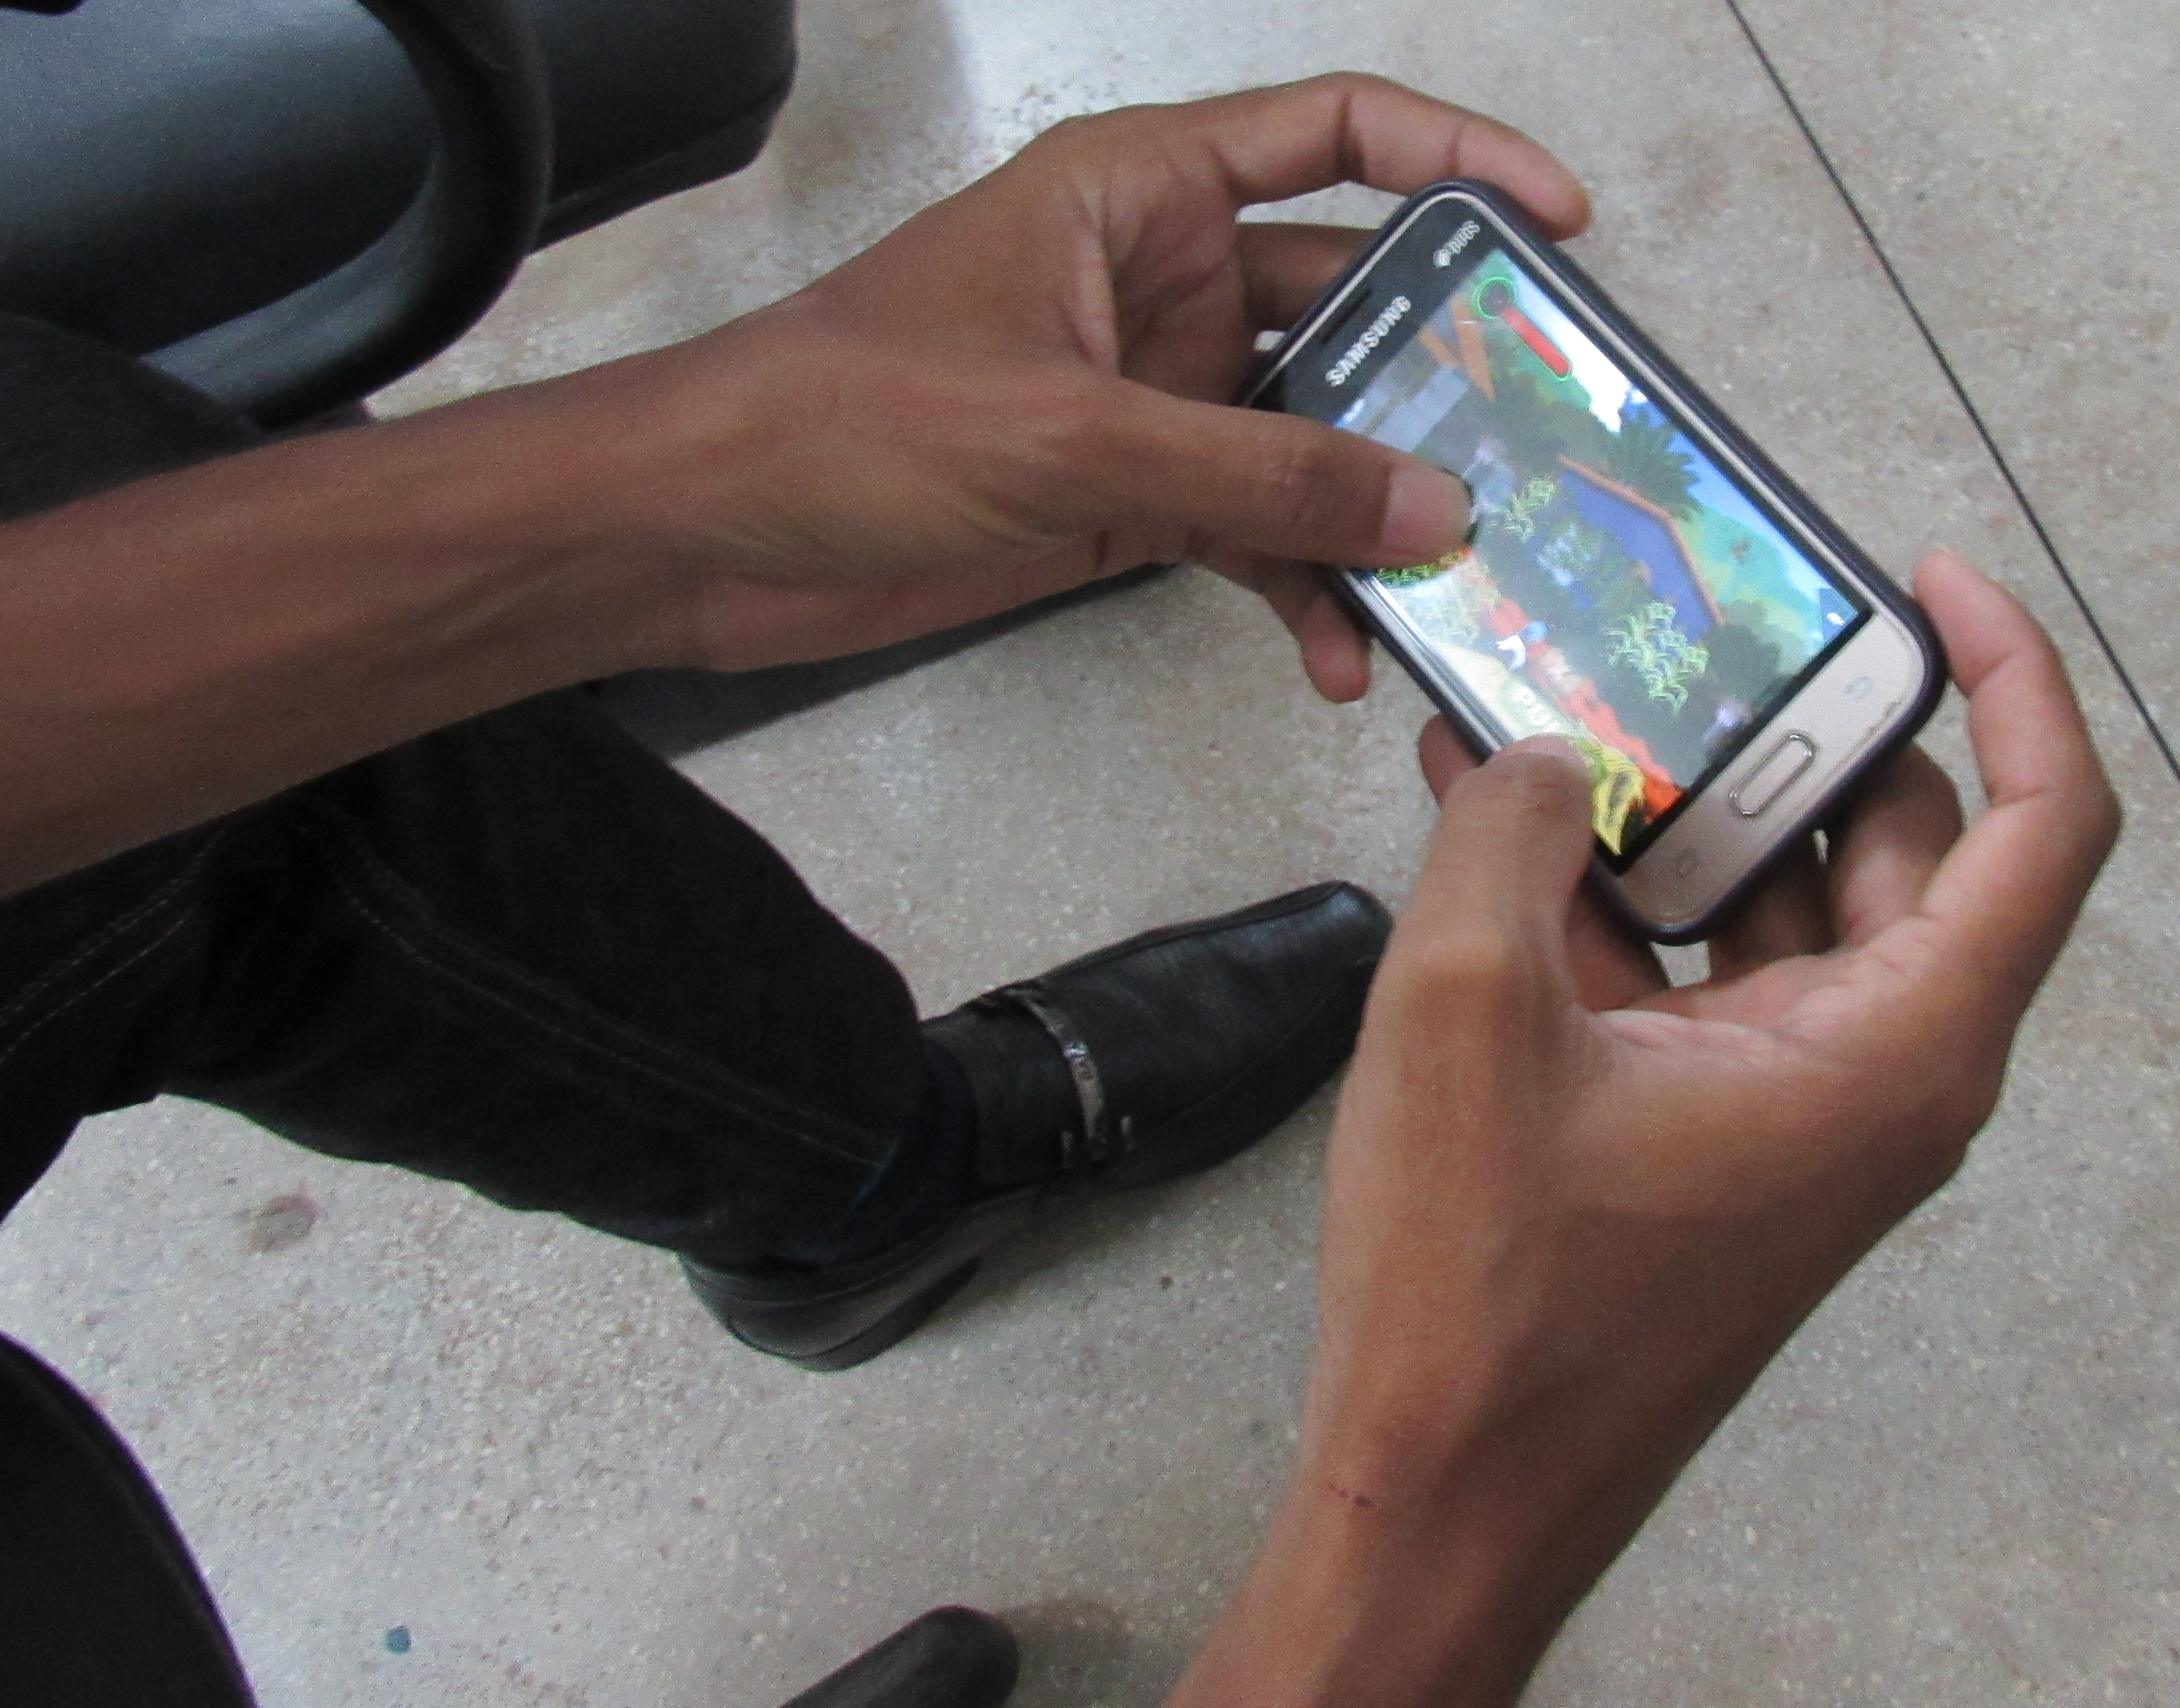
\includegraphics[width=0.62\textwidth]{figuras/aluno_teste.jpg}
	\label{fig:avaliacao-aluno}
	{\fonte{O Autor (2018)}}
\end{figure}